\documentclass[a4paper,12pt]{article}

\usepackage{graphicx}
\usepackage{url}
\usepackage{xcolor}

\setlength{\parskip}{\baselineskip}%
\setlength{\parindent}{0pt}%

\begin{document}

\title{Large Scale Sentiment Analysis of Tweets }%replace with the appropriate homework number
\author{
	James Tan Juan Whei 40161156\\
	Vithushon Maheswaran 27052715\\
	Saeedeh Moghimi 40184202\\
	AmirAli Sabaghpourfard 40185709\\
	\\Concordia University
}
\maketitle

\begin{abstract}
The aim of this paper is to analyze the sentiments of tweets in a specific duration of time. We have used a library called snscrape\cite{snscrape} to
scrape approximately 10GB worth of tweets and Apache spark and BigQuery to store and analyze the data.
The library we have used to classify the tweets is called ClassifierDLModels. The results show the percentage of sentiment in
tweets during a certain time and also as there was a shooting in this period, charts show how much sentiment of fear increased
from one day to another. Finally, we conclude the results and show the charts and results.
\end{abstract}

\section{Introduction}
This project aims to apply distributed system concepts with real applications, such as NoSQL systems for big data,
and demonstrate the power of distributed systems in extracting and analyzing the general sentiment expressed in a large
data set of tweets, and detecting emotions and cyberbullying using pretrained Spark NLP DL classifiers.
Emotions identified include Joy, Surprise, Fear, and Sadness while detecting Racism, Sexism, or Neutral tweets.

\section{Tools and Technologies}
Given the large dataset, approximately 10 GB of scrapped tweets, we chose google cloud storage.
Google Cloud Storage is a RESTful online file storage web service for storing and accessing data on a Google Cloud
Platform infrastructure. The service combines the performance and scalability of the cloud with advanced
security and sharing capabilities, all at no cost to a user using less than 15 GB of cloud space for free.

Furthermore, Big Query was chosen to store the tweets as tabular data in datasets and tables. BigQuery is a data warehouse
and a SQL Engine that enabled ease of data import due to its compatibility with GCS. It's also an affordable big data
warehouse, where the first Terabyte of data processed each month is free.

In order to process our data and draw insight from processed tweets, we used Apache Spark, an open-source unified analytics engine for
large-scale data processing. To run Apache Spark, we used Dataproc, given the fast, easy-to-use, and fully managed cloud
service for running Apache Spark clusters in a simpler, more cost-efficient way. It helps you create clusters quickly,
manage them easily, and save money by turning clusters off when you don't need them.

\subsection{GCS}
GCS, or Google Cloud Storage\cite{GCS}, is an object storage service on the Google Cloud. GCS stores a variety of data
(objects) in containers called buckets. GCS offers different types of classes like Standard, Nearline, Coldline, and
Archive, which makes a difference in price and availability\cite{GCSClasses}.

For this project, we used GCS to store CSV files before loading them into  BigQuery. To decrease time consumption, we uploaded all the CSV files to
a Standard class GCS bucket, and then BigQuery ingested the data directly from there. In order to upload files to GCS, we used this command:

\# gsutil cp *.csv gs://tweets\_bucket\_comp6231/

\subsection{BigQuery}
Google BigQuery is a cloud-native, enterprise-grade data warehouse. BigQuery was first made available as a service in
2010 and became generally available in November 2011. Since its debut, BigQuery has developed into a more affordable,
fully-managed data warehouse that can process petabyte-scale datasets with lightning-fast interactive and ad-hoc queries.
BigQuery is now more functional thanks to its integration with a number of Google Cloud Platform (GCP) services and
third-party tools.

BigQuery, or more specifically data warehouse as a service, is serverless. No servers or database software needs to be
installed or managed. The BigQuery service maintains the infrastructure, including scalability and high availability,
as well as the underlying software. The pricing structure is fairly straightforward: every TB of data costs \$5 to process. BigQuery reveals a simple client interface that enables users to run interactive queries.


BigQuery is built on  Dremel\cite{Dremel}, which has been operating internally at Google since 2006. Dremel is Google's
ad hoc interactive query system for analyzing read-only nested data. The first Dremel paper was published in 2010.
At the time of publication, Google was running multiple instances of Dremel ranging from tens to thousands of nodes.

BigQuery and Dremel have the same underlying architecture. By integrating Dremel columnar storage and tree architecture,
BigQuery offers unprecedented performance. But BigQuery is much better than Dremel. Dremel is just an execution engine for BigQuery. In fact, the BigQuery service uses Google's innovative technologies such as Borg\cite{Borg}, Colossus, Capacitor, and Jupiter.

A BigQuery client (usually the BigQuery web UI or bg command line tool or REST API) interacts with the Dremel engine
through the client interface. Borg, Google's large cluster management system, allocates computing capacity to Dremel
jobs. The Dremel job reads data from Google's Colossus file system over the Jupiter network, performs various SQL
operations, and returns the results to the client. Dremel implements a multi-level server tree to execute queries.

The most expensive part of any big data analytics platform is almost always disk I/O. BigQuery stores data in a columnar
format called capacitor\cite{StoringDremel} . As you can imagine, each field of a BigQuery table i.e. column is stored in
a separate Capacitor file which enables BigQuery to achieve a very high compression ratio and scan throughput.

\subsection{Dataproc and Spark}
\label{sec:spark}
Dataproc is a managed framework that runs on the Google Cloud Platform and ties together several popular tools for processing data.
We used it to run Apache Spark clusters. It's easy to use and relatively fast, as you can spin up a cluster in about 90 seconds.
It’s cheaper than building your own cluster because you can spin up a Dataproc cluster when you need to run a job and
shut it down afterward, so you only pay when jobs are running. Dataproc is priced at only 1 cent per virtual CPU in your
cluster per hour. Conveniently, it’s integrated with other Google Cloud services, including Cloud Storage, BigQuery, and
Cloud Bigtable, making it easy to transfer our data. Due to performance considerations as well as the high reliability of
storage attached to Dataproc clusters, the default replication factor is set at 2.

Compute Engine Virtual Machine instances (VMs) in a Dataproc cluster, consisting of master and worker
virtual machines, require full internal IP networking cross connectivity. The default Virtual Private Cloud network provides
this connectivity and offers native Internal TCP/UDP Load Balancing and proxy systems for Internal
HTTP and HTTPS Load Balancing.

Dataproc clusters can be created using the Google Cloud Platform console, or alternatively to create a Dataproc cluster
on the command line, run the Cloud SDK gcloud dataproc clusters create command locally in a terminal window or in
Cloud Shell. Refer to section 7 - Code to see our code for cluster creation.

Basic requirements for cluster creation include specifying a cluster name, region (global or a specific region for the cluster), and
connectivity consisting of the number of master and worker nodes.

gcloud dataproc clusters create cluster-name \
--region=region

The above command creates a cluster with default Dataproc service settings for your master and worker virtual machine
instances, disk sizes, and types, network type, region and zone where your cluster is deployed, and other cluster settings.

In order to set attributes specific to the required resource, you can specify the specific values against the
the flag you want to modify.

The following flags were used to specify unique attributes for the resources of our VMs:

Type of machine to use for worker nodes.

--worker-machine-type n1-standard-8 \

The size of the boot disk, in our case a 128 GB disk.

--master-boot-disk-size=128GB \
--worker-boot-disk-size=128GB \

We used the default number of master nodes (1 node), however, to specify otherwise when High Availability is critical,
the number of master nodes in the cluster can be changed to 3.

--num-masters=1

For the number of worker nodes in the cluster, we only used 2 worker nodes.

--num-workers=2 \

To submit a job to a Dataproc cluster, run the gcloud CLI gcloud dataproc jobs submit command locally
in a terminal window or in Cloud Shell.

\section{Dataset}
\label{sec:dataset}
We relied heavily on the snscrape \cite{snscrape} library to scrape tweets. We filtered for tweets that were in the
English language only. Approximately 1000000 tweets were scraped for each day between 2022-05-01 and 2022-07-12. The
tweets were then saved in Google Cloud Storage.

\section{Processing of Data}
As mentioned in Section \ref{sec:spark}, we define the processing of the data as a Spark job. The steps involved in the
job are illustrated in Figure \ref{fig:data-processing-pipeline} and will be further elaborated on in the subsequent
sections. Our processing pipeline relies heavily on the Spark NLP library\cite{SparkNLP}.

\begin{figure}[h]
\centering
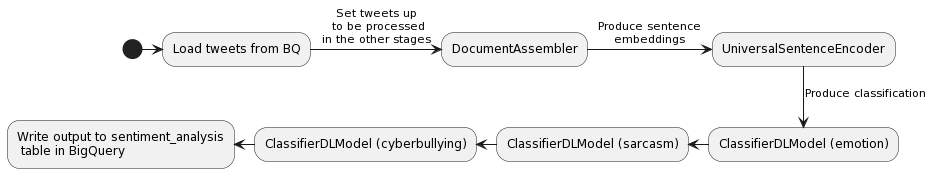
\includegraphics[width=\textwidth]{data-processing.png}
\caption{The processing pipeline}
\label{fig:data-processing-pipeline}
\end{figure}

\subsection{Data Ingestion}
In order to use data stored in BigQuery as an input to our Spark job, we used the Spark BigQuery
connector\cite{BigQueryconnector}. The Spark script reads from a table that contains all the tweets that were
procured as described in Section \ref{sec:dataset}.

Each run of the Spark job would typically be executed on 4-5 days' worth of tweets as we discovered that the Spark jobs
had a tendency of failing when working with larger amounts of data. This was true even when the CPU and memory
utilization of the worker nodes were relatively healthy and thus should be further investigated.

\subsection{Document Assembler}
The first step of the pipeline is the \texttt{DocumentAssembler}\cite{DocumentAssembler}. This prepares the data into
a format that is processable by Spark NLP and is essentially the entry point for every Spark NLP pipeline.

\subsection{Generation of Sentence Embeddings}
\label{sec:sentence-embeddings}

We generate sentence embeddings by leveraging a Universal Sentence Encoder\cite{semanticSimilarity} made available by
Tensorflow. The output of this stage is a 512-dimensional vector that semantically captures the meaning of each tweet.
This is the basis upon which the downstream classification algorithms build on.

\subsection{Sentiment Classification}
To actually use the embeddings described in the previous section, we utilize ClassifierDLModels\cite{ClassifierDLModel}
to classify the tweets. Each ClassifierDLModels essentially assigns a label to each tweet. To identify the emotion,
presence of cyberbullying and presence of racism in each tweet, we use the \texttt{classifierdl\_use\_emotion},
\texttt{classifierdl\_use\_cyberbullying} and \texttt{classifierdl\_use\_sarcasm} pretrained models respectively.

The emotion classifier produces the values \texttt{sadness}, \texttt{joy}, \texttt{love}, \texttt{anger},
\texttt{fear} and \texttt{surprise}. The cyberbullying classifier produces the values \texttt{neutral},
\texttt{racism} and \texttt{sexism}. The sarcasm classifier produces the values \texttt{sarcasm} and \texttt{normal}.

\subsection{Storing of Output}
The output is then stored in a separate table in BigQuery. Note that the BigQuery Spark connector is once again used here, thus allowing the output of a Spark job to be appended directly to a BigQuery table.

\section{Results}
To visualize the general sentiment expressed in tweets, detected emotions, and cyberbullying, we used Jupyter notebook to
display and provide the functionality to query the data interactively.

Emotions identified include Joy, Surprise, Fear, Sadness while detecting Racism, Sexism, or Neutral tweets.
\subsection{Sample Output: Query of Racist Tweets}
Below you see the sample output for a query on racist tweets between the 1st and 4th of May, 2022. Note, that the data output
has been cropped to 5 tweets for convenience.

\begin{figure}[h!]
\centering
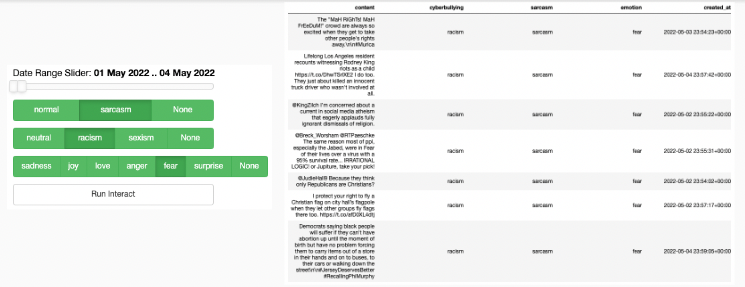
\includegraphics[width=\textwidth]{racism.png}
\caption{Sample Query: General Sentiment Over Time}
\label{fig:Query-Racist-Tweets}
\end{figure}

\subsection{Sample Output: General sentiments}
Below is another visualization provided using a Jupyter notebook, that enables us to visualize the emotions of tweets over time.
Interestingly, you can see the spike of fear on May 24th, 2022.

\begin{figure}[h!]
{\centering
	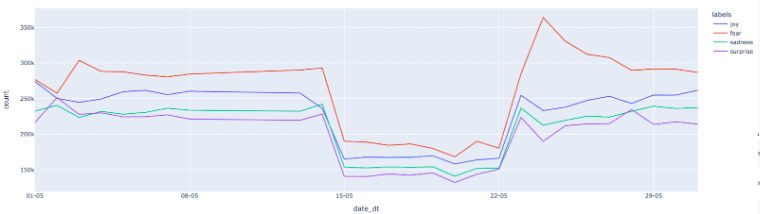
\includegraphics[width=\textwidth]{graph.png}
	\caption{Sample Query: General Sentiment Over Time}
	\label{fig:Emotion-Time-Query}
}
	\vspace{5mm} %5mm vertical space
By using our interactive tweet-emotion visualizer, we can
observe the emotion of the general users on Twitter, and here we unfortunately notice that a shooting had taken place
on the 24th of May, 2022.
	{
	\centering
	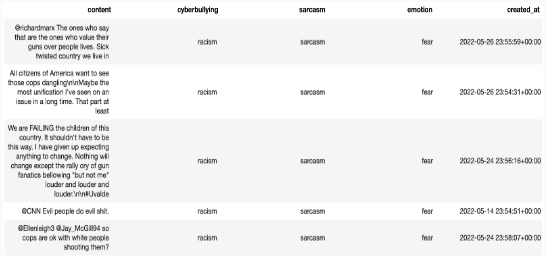
\includegraphics[width=\textwidth]{graphTweets.png}
	\caption{Sample Query: Fear}
	\label{fig:Fear-Query}
}
\end{figure}

\section{Future Work}
An idea that we originally had was to run an unsupervised clustering algorithm on the sentence embeddings produced in Section \ref{sec:sentence-embeddings}. The clustering algorithm that we had in mind was DBScan\cite{Ester96adensity-based}, with the objective of clustering tweets with similar topics. Unfortunately, we were not able to find a satisfactorily efficient implementation of the algorithm to employ with Spark. Due to the size of our dataset and the high number of dimensions of the embeddings, an efficient implementation was crucial to the success of this idea. Given that we had limited resources, we were forced to abandon this idea, however, it should be revisited in the future by implementing our own version of the DBScan algorithm.

\section{Code}
The code to reproduce our project may be found in our Github repository \cite{Githubrepository}.

\section{Team-Work}
Given the limited time, the project scope was distributed amongst each team member, and logically split into three distinct
areas as follows:

1. Data storage\\
2. Data processing\\
3. Data visualization

Saeedeh was responsible for storing our raw data into BigQuery Table.
James and Vithu were responsible for processing the data.
AmirAli was responsible for the visualization of the data.

\section{Conclusion}
We explored various distributed applications that stored, processed, and analyzed data, while considering multiple
factors such as performance, cost, ease of use, availability, etc. This project has demonstrated the convenience
of such applications based on Google Cloud architecture. Although our data processing was not as compute-intensive
to warrant the use of the clusters chosen, the project has demonstrated the capabilities of distributed systems by
extracting, analyzing, and storing the general sentiments expressed by the large data set of tweets.

\nocite{*}

\bibliographystyle{abbrv}
\bibliography{main.bib}

\end{document}  
